\chapter{Stromal and Oncogenic Regulation of Colonic Stem Cell Polarisation}
\label{04seq}

\section{Introduction}


% Given the well-known biology of the murine small intestine at the transcriptome level21, we can analyse the SI LGR5s to characterise the different subpopulations within the epithelial organoids and cross-validate the results with in vivo scRNA-seq studies and the mass cytometry results discussed above11. In a similar fashion, we also aim to characterise the colonic organoids and the stromal and immune compartments that form the TME in the heterocellular cultures. Unlike mass cytometry, which requires tailored panels of antibodies reaching only into a few dozens, with scRNA-seq we will be able to characterise thousands of genes at once in the organoids, fibroblasts, and macrophages. 
% Leveraging the publicly available ligand-receptor databases mentioned in the background section, data from the scRNA-seq experiments will be used to identify the ligands and receptors expressed in the colonic heterocellular organoid cocultures. 
% The cell communication information gathered this way can then be summarised as signalling pathways that define and connect the different populations of cells. Furthermore, the study of this interactome would aid towards understanding the interplay between the CRC organoid model and its TME. This can be achieved by comparing the cell communication results with the intracellular PTM signalling described in Qin et al. 2020 and seeing how cellular communications change in cultures mimicking an oncogenic setting.

As presented in Chapter \ref{01intro}, the colonic epithelium is a highly heterogeneous system with multiple specialised cell types. Supported by the \emph{Lgr5}\textsuperscript{+} colonic stem cells (CSCs) of the crypt, its homeostatic regulation relies on intrinsic and extrinsic cues, the latter of which predominately come from the stromal compartment. In the context of colorectal cancer (CRC), and under the classical progression model \cite{fearon_genetic_1990}, oncogenic mutations targeting \textit{Apc}, \textit{Kras}, \textit{Braf}, \textit{Smad4}, and/or \textit{Trp53} constitute intrinsic cues that are sufficient to induce a highly proliferative crypt-progenitor phenotype (proCSC) in cancer cells \cite{van_de_wetering_-catenintcf-4_2002}.
Therefore, in both the healthy colon and CRC a compartment of epithelial cells is maintained in a stem-like state, although by different mechanisms. 

This shared crypt-progenitor phenotype actually represents a broader compartment encompassing more than the canonical LGR5\textsuperscript{+} CSCs; with recent studies describing the existence of the \emph{Clu}\textsuperscript{+} revival stem cell state (revCSC). Reminiscent of foetal-like states, the revCSC compartment has been described as a small and non-hyperproliferative compartment involved in tissue regeneration after injury and suggested as a drug-tolerant persister state in CRC. 

However, the mechanisms of regulation between the different stem cell states largely remain unclear.
Involvement of cell extrinsic cues in the form of stroma-secreted ligands, coupled with the association of the TME with CRC progression, suggest that they must also pay a role in regulating the colonic epithelia. The cell extrinsic cues involve signalling pathways that overlap with those affected by the oncogenic mutations \colorbox{yellow}{Reference here\cite{sphyris_subversion_2021}, also spell out pathways?}, indicating a competition between intrinsic and extrinsic cues to regulate epithelial polarisation might take place during oncogenesis.

% Canonically, both stromal WNT/R-Spondin-1 ligands and APC-loss hyper-activate \textbeta-catenin signalling, whereas EGF and KRAS/BRAF mutations stimulate the MAPK pathway \cite{sphyris_subversion_2021}.

Thus, single-cell omic technologies are perfectly placed to understand polarisation of the epithelial compartment at a broader level and reveal the regulation of cell fates by competing cues.

In this Chapter I will explore via scRNA-seq how cell extrinsic and intrinsic cues co-regulate colonic epithelial fate using a heterocellular organoid culture system with both environmental and oncogenic perturbations. I will first characterise the different populations found in the heterocellular cultures, identify the different epithelial cell states and their compositional changes in response to intrinsic and extrinsic cues. Cellular dynamics approaches will reveal our understanding of the balance regulating the proCSC and revCSC states, and cell-cell communication analysis will suggest putative mechanisms of regulation. Finally, the findings will be contextualised with the broader literature leveraging published gene signatures.

The work presented here is part of Qin \& Cardoso Rodriguez et al. 2023 \cite{cardoso_rodriguez_single-cell_2023}, where it is shown accompanied with mass cytometry analyses carried out by Dr. Xiao Qin and whose results validate the scRNA-seq findings and shed light on the mechanisms of epithelia stem cell polarisation in this shared landscape.


\subsubsection{Figure on experimental design, with the 2 axes of perturbation}

\begin{figure}
    \centering
    \includegraphics{04seq/figs/4SEQ_ExpDesign.png}
    \caption{\textbf{A)} Multivariate scRNA-seq experimental design. WENR ligands were removed from all experimental conditions except for the niche factor control to ensure cell-cell signalling was not dominated by exogenous recombinant proteins (see Methods). \textbf{B)} Single-cell PHATE embedding illustrating epithelial cells, fibroblasts, and macrophages. \textbf{C)} PCAs of epithelial, fibroblast, and macrophage transcriptomes regulated by by organoid genotype and microenvironment. WENR, WNT3A, EGF, Noggin, and R-Spondin-1.}
    \label{fig:4exp}
\end{figure}

\colorbox{yellow}{ADD fib and mac reference}
To directly compare how CRC oncogenic mutations and stromal cells regulate colonic epithelial differentiation, I performed a multivariate scRNA-seq analysis of wild-type (WT), \textit{shApc} (A), \textit{shApc} and \textit{Kras\textsuperscript{G12D/+}} (AK), and \textit{shApc}, \textit{Kras\textsuperscript{G12D/+}} and \textit{Trp53\textsuperscript{R172H/–}} (AKP) colonic organoids, in monoculture or co-cultured with colonic fibroblasts and/or macrophages (Figure \ref{fig:4exp}A). Fibroblasts are established regulators of intestinal epithelia \cite{roulis_fibroblasts_2016} and macrophages are the most profuse leukocytes in the colon \cite{isidro_colonic_2016}. A condition with WT organoids cultured with exogenous WNT3A, EGF, Noggin, and R-Spondin-1 (WENR) (commonly used to grow colonic organoids) was included as a defined mesenchymal niche factor control. 

Following data acquisition and initial preprocessing steps (see Chapter \ref{02methods}), epithelial cells, fibroblasts, and macrophages were jointly embedded in an integrated space and visualised by PHATE (Potential of Heat-diffusion for Affinity-based Trajectory Embedding) \cite{moon_visualizing_2019}. This embedding resolves the three distinct cell types as shown by expression of levels of canonical cell type markers (Figure \ref{fig:4exp}B). 
Cell-type-specific transcriptional changes were referenced against each the control monoculture conditions (WT organoids for the epithelial cells) using the EMD score (see \ref{02methods}, and then summarised using PCA (Figure \ref{fig:fig1}C). Epithelial transcriptomes are differentially regulated by both CRC mutations (PC1, 26\%) and microenvironmental cues (PC2, 22\%), with A, AK, and AKP mutations progressively dysregulating their transcriptomic profiles. However, we found fibroblasts can only regulate WT and A epithelial cells (Figure \ref{fig:fig1}C). Although WENR ligands are thought to mimic a healthy stromal niche \cite{mahe_establishment_2013}, WT organoids + WENR ligands transcriptionally align with AK mutant organoids (not WT+fibroblasts as might be expected), indicating this widely used colonic organoid culture media induces a partial CRC-like transcriptome in WT epithelia (Figure \ref{fig:fig1}C).

% Colonic fibroblasts clustered into CD34\textsuperscript{hi} and CD34\textsuperscript{lo} subpopulations mimicking \textit{in vivo} stromal heterogeneity \cite{stzepourginski_cd34_2017, karpus_colonic_2019} (Figure \ref{suppfig:figs1}A). CD34\textsuperscript{hi} and CD34\textsuperscript{lo} fibroblasts did not differentially regulate colonic epithelia (Figure \ref{suppfig:figs1}B) and were subsequently treated as a heterogenous mesenchymal population. We found fibroblast and macrophage transcriptomes were only regulated by co-culture with heterotypic cells but not altered by epithelial genotypes (Figures \ref{fig:fig1}C, \ref{suppfig:figs1}C-D). 

\colorbox{yellow}{NEDD TO ADD SUP FIG OF HEATMAPS}

Colonic fibroblast cells resolved into CD34\textsuperscript{hi} and CD34\textsuperscript{lo} subpopulations mimicking \textit{in vivo} stromal heterogeneity \cite{karpus_colonic_2019} (Figure \ref{suppfig:figs1}A). CD34\textsuperscript{hi} and CD34\textsuperscript{lo} fibroblasts did not differentially regulate colonic epithelia (Figure \ref{suppfig:figs1}B) and were subsequently treated as a heterogenous mesenchymal population. Bone marrow macrophages on the other hand presented as a continuum of cells aligned along and axis of inversely correlated expression of complement genes (like \emph{C1q}) and \emph{Hmox1}, see \ref{fig:4exp}), possibly indicating inflammation-related roles to be a major driver of heterogeneity within the macrophage cells \cite{naito_heme_2014}. However, we found that fibroblast and macrophage transcriptomes and compositional make-up were only regulated by co-culture with heterotypic cells but not altered by epithelial genotypes (Figures \ref{fig:fig1}C, \ref{suppfig:figs1}C-D). 


\section{Organoids recapitulate colonic epithelial cell states}

\subsubsection{Figure on Integrated object DR, and expression of cannonical markers in control condition}
\begin{figure}
    \centering
    \includegraphics{04seq/figs/4SEQ_INTctrl.png}
    \caption{\textbf{D)} PHATE embedding of 29,452 epithelial cells from the 17 organoid conditions coloured by cell-type clusters. CSC, colonic stem cell. proCSC, hyper-proliferative CSC. revCSC, revival CSC. DCS, deep crypt secretory cell. TA, Transit amplifying cell. \textbf{B)} Single-cell PHATE embeddings of epithelial cells from WT, WT+Fibroblasts, WT+WENR, and AK organoids coloured by cluster and overlaid with single-cell density.}
    \label{fig:4intepi}
\end{figure}

Epithelial cells from all conditions were integrated by reciprocal PCA (RPCA) \cite{hao_integrated_2021}, projected onto a shared PHATE embedding, and clustered into multiple cell-fates, including stem populations, transit amplifying (TA) cells, cells under ER stress, goblet and deep crypt secretory (DCS) cells, and early or late enterocytes (Figure \ref{fig:fig1}D). 

Identify via expression of canonical markers \colorbox{yellow}{Table of markers}. REsolves stem, secretory and absorptive compartments. nice progression/reoslution in absorptive compartment but unable to discern between the different secretory populations. Data on similar SI organoids also presented with the same quirck (so perhaps lmitation of the organoid model system). Stem compartment broad and overlapst with TA cells. ER stress adjacent to it with clear ER stress response gene expression.

Integrated space can then be seolved on individual conditons, chosen 4 extremes of the experimental matrix we see trends of polarisation changes occuring via density plots.


\section{Oncogenic mutations and fibroblasts polarise epithelia towards distinct stem cell fates}

Differential abundance testing \cite{dann_differential_2022} of co-culture and CRC monoculture conditions against WT monocultures revealed that fibroblasts, macrophages, and CRC mutations have markedly different effects on epithelial cell-fate determination (Figure \ref{fig:fig1}F-H). 

\begin{figure}
    \centering
    \includegraphics{04seq/figs/4SEQ_DA.png}
    \caption{\textbf{F)} Epithelial PHATE overlaid with differentially abundant (DA) neighbourhoods in WT organoid + fibroblast co-cultures compared with WT organoid monocultures. \textbf{G)} Epithelial PHATE overlaid with DA neighbourhoods in AK/AKP organoid monocultures compared with WT organoid monocultures. \textbf{H)} Dot plot of epithelial clusters across organoid cultures coloured by log fold-change (Log FC) in neighbourhood abundance and sized by the number of neighbourhoods detected.}
    \label{fig:4da}
\end{figure}

Fibroblasts enrich a distinct stem cell population characterised by high expression of epithelial progenitor genes \textit{Clu}, \textit{Sox9}, \textit{Cd44}, and \textit{Cldn4} (Figures \ref{fig:fig1}I). 

In contrast, A, AK, and AKP mutations progressively polarise epithelia towards a hyper-proliferative colonic stem cell-fate, hereafter named proCSC (Figure \ref{fig:fig1}G, H). proCSCs express \textit{EphB2}, \textit{Birc5} (\textit{Survivin}), \textit{Lrig1}, \textit{Hmgb2}, and \textit{Rrm2} and are highly mitotic (\textit{Stmn1\textsuperscript{+}}, \textit{Mki67\textsuperscript{+}}, and \textit{Ccnb1\textsuperscript{+}}) (Figure \ref{fig:fig1}I). 

Both revCSC and proCSC are present in WT organoids at low levels alongside traditional \textit{Lgr5\textsuperscript{+}} colonic stem cells, hereafter named CSC (Figure \ref{suppfig:figs2}B). We found CSC are also enriched by A, AK, and AKP genotypes, but to a lesser extent than proCSC.

\begin{figure}
    \centering
    \includegraphics{04seq/figs/4SEQ_DE.png}
    \caption{\textbf{I)} Gene expression signatures of epithelial clusters.}
    \label{fig:4de}
\end{figure}


We found that fibroblasts can only induce revCSC in WT and \textit{shApc} epithelia, but not when cells contain both \textit{shApc} and \textit{Kras\textsuperscript{G12D/+}} (Figure \ref{fig:fig1}H). Conversely, proCSCs are enriched in all A, AK, and AKP organoids irrespective of fibroblasts or macrophages, suggesting oncogenic mutations are dominant over microenvironmental signalling. WENR ligands hyper-polarise WT epithelia towards all stem and TA cell-types, with very few cells retaining secretory or absorptive identities (Figures \ref{fig:fig1}H-I, \ref{suppfig:figs2}B). WT epithelia also show higher RNA velocity vector lengths relative to CRC cells (Figure \ref{suppfig:figs2}C-D), suggesting that oncogenic mutations reduce epithelial plasticity. While macrophages can alter epithelial gene expression (Figure \ref{fig:fig1}C), macrophages do not regulate the abundance of epithelial cell-types (Figure \ref{fig:fig1}H). In summary, multivariate scRNA-seq revealed that fibroblasts, CRC mutations, and WENR ligands polarise epithelia towards a de-differentiated progenitor state – with fibroblasts and oncogenes inducing distinct revCSC and proCSC fates.



\subsubsection{Figure on signalling entropy, RNA velocity changes, and CellRank sinks}

\begin{figure}
    \centering
    \includegraphics{04seq/figs/4SEQ_Dynamics.png}
    \caption{\textbf{E)} Epithelial PHATE coloured by CCAT score and overlaid with velocity streams (arrows). \textbf{C)} Single-cell PHATE embeddings coloured by RNA velocity vector lengths. \textbf{D)} RNA velocity vector lengths of organoid conditions (Games-Howell pairwise test with Holm-adjusted \textit{p}-values). \textbf{E)} CCAT scores of epithelial clusters.}
    \label{fig:4dyn}
\end{figure}

Stem clusters contain high signalling entropy (indicative of pluripotency) \cite{teschendorff_singlecell_2017} and act as origins for RNA velocity streams \cite{bergen_generalizing_2020} that transition towards differentiated cells (Figures \ref{fig:fig1}E, \ref{suppfig:figs2}E).

Origin of velocity seems to be the proCSC state. Then going towards differentiated states in WT monoculture. However, addition of fibroblasts orWENR ligands to organoids polarises towards revCSC. In cancer, heavily altered differentation landscape, but still proCSC remain the source.

\section{Oncogenic mutations block fibroblast to epithelia signalling}

As epithelial differentiation cannot be regulated by fibroblasts in the context of \textit{shApc} and \textit{Kras\textsuperscript{G12D/+}} (Figures \ref{fig:fig1}H, \ref{fig:fig2}C), we hypothesised oncogenic mutations might disrupt stromal-epithelial signalling. To test this, we performed ligand-receptor cell-cell communication analysis \cite{jin_inference_2021} of WT, A, AK, and AKP organoid+fibroblast co-culture scRNA-seq datasets. 

Given their established role in microenvironmental cell-cell communication, fibroblasts unsurprisingly demonstrate high 'outgoing' signalling (i.e., express numerous ligands and extracellular matrix (ECM) components). By contrast, WT epithelia display a dominant 'incoming' signalling potential (i.e., express many receptors) (Figure \ref{fig:fig4}A). This dichotomy suggests that heterocellular signalling in the healthy colon is largely unidirectional from fibroblasts to epithelial cells. We found that revCSC and the closely affiliated TA 1 and TA 2 clusters are responsible for much of the 'incoming' signalling potential of WT epithelia, indicating these cell-types are hyper-sensitive to cell-extrinsic regulation by fibroblasts. In contrast, proCSC are the least receptive of all epithelial cells, suggesting proCSC are more reliant on cell-intrinsic signalling (Figure \ref{fig:fig4}A). 

Cell-cell communication analysis revealed that fibroblasts form putative paracrine and juxtacrine interactions with WT and A cells, which are often lost in AK and AKP genotypes (Figure \ref{fig:fig4}B). For example, WT and A organoids show intact NRG1, EREG, IGF, and TGF-\textbeta\hspace{0.1cm}signalling with fibroblasts, but these cell-cell interactions are undetectable in AK and AKP cells, due to the downregulation of epithelial signal receptors (Figures \ref{fig:fig4}B-C, \ref{suppfig:figs5}A-C).

% Ligand-receptor analysis is increasingly used to generate putative cell-cell communication models in heterocellular systems \cite{dimitrov_comparison_2022}, yet these computational hypotheses are rarely experimentally validated. To functionally test how oncogenic mutations regulate stromal-epithelial communication, we performed a systematic TOB\textit{is} MC study of epithelial differentiation, cell-state, and PTM signalling in WT, A, K, KP, AK, and AKP organoids treated with stromal ligands identified by ligand-receptor analysis as WT homeostatic regulators (WNT5A, SEMA3A, TGF-\textbeta1, TGF-\textbeta2, IGF, NRG1, EREG, and OPN (\textit{Spp1})) (Figure \ref{fig:fig4}B-C).



\subsubsection{Figure on cell-cell communication analysis}

\begin{figure}
    \centering
    \includegraphics{04seq/figs/4SEQ_CC.png}
    \caption{\textbf{Oncogenic Mutations Disrupt Stromal-epithelial Communication.} \textbf{A)} Outgoing and incoming communication probability (interaction strength) from fibroblasts to epithelia across organoid genotypes. \textbf{B-C)} Predicted paracrine and juxtacrine communication summarised at the pathway and ligand-receptor interaction level. \textbf{A)} Average scaled expression of ligands (expressed by fibroblasts) and receptors (expressed by epithelia) across organoid genotypes. \textbf{B)} Ligand expression (\textit{UCell} scores) by fibroblasts in co-cultures across organoid genotypes (Games-Howell pairwise test, n.s not significant). \textbf{C)} Receptor expression (\textit{UCell} scores) by epithelia in co-cultures across organoid genotypes (Games-Howell pairwise test with Holm-adjusted \textit{p}-values).}
    \label{fig:}
\end{figure}

\section{Characterisation and relevance of proCSC and revCSC}




\subsubsection{Figure on stem signatures and key signalling pathways}

\begin{figure}
    \centering
    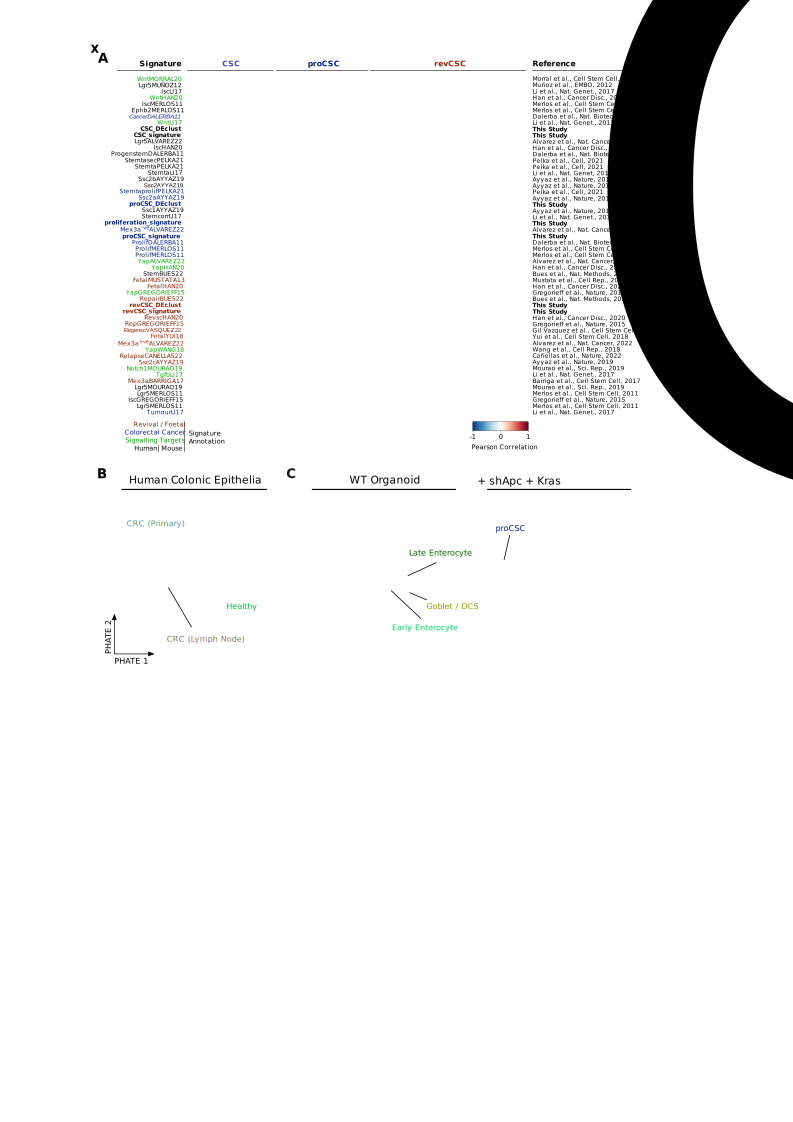
\includegraphics{04seq/figs/4SEQ_StemSign.png}
    \caption{\textbf{Epithelial Stem Cell Signatures. Related to Figure 1.} \textbf{A)} Comparison of gene signatures of CSC, proCSC, and revCSC identified in this study with published stem cell signatures.}
    \label{fig:}
\end{figure}


These fibroblast-induced stem cells are transcriptionally similar to 'foetal' \cite{mustata_identification_2013, yui_yap_2018} or 'revival' stem cells (revSCs) \cite{ayyaz_singlecell_2019} of the small intestine (\ref{suppfig:figs2}A) and are hereafter referred to as 'revival colonic stem cells' (revCSC).
In addition, proCSCs are transcriptionally comparable to stem cells observed in mouse and human CRC (Figure \ref{suppfig:figs2}A). CSC gene signatures are less common in CRC (Figure \ref{suppfig:figs2}A).


\section{Conclusions}

revealed that fibroblasts and oncogenic mutations induce distinct epithelial stem cell-fates in colonic epithelia. We find that fibroblasts polarise epithelia towards slow-cycling CLU\textsuperscript{+} revival stem cells \colorbox{yellow}{CELLCHAT TARGETSvia TGF-\textbeta1 and YAP}, whereas APC-loss, KRAS\textsuperscript{G12D}
%, and/or exogenous Epiregulin (EREG) 
Oncogenes shift cells towards a LRIG1\textsuperscript{+} hyper-proliferative fate that is dependent on PI3K signalling. APC-loss and KRAS\textsuperscript{G12D} collaboratively block cell-extrinsic regulation of epithelial plasticity by interrupting stromal-epithelial communication, trapping CRC cells in a cancerous state.

Exogenous WNT and EGF ligands can polarise the epithelium towards both states, at the expense of the differentiated cell states. Yhe paired analysis on Qin \& Cardoso Rodriguez et al 2023 shows how CRC organoids can still access revival stem cells, but this requires high cell-extrinsic activation of YAP via TGF-\textbeta1 in parallel with reduced PI3K signalling. 

These results demonstrate that colonic epithelia exist on a continuous differentiation landscape where oncogenic mutations and stromal cues compete for epithelial identity -- but oncogenes eventually dominate by blocking the stromal regulation of cell-fate plasticity. 


% Single-cell technologies can describe cell-type-specific regulation of differentiation and cell-cell communication \cite{qin_deciphering_2021, fleck_inferring_2022, bues_deterministic_2022}. In this study, we utilised both multiplexed scRNA-seq and high-throughput MC to functionally map how oncogenic mutations and stromal cues co-regulate colonic epithelia across a continuous polarisation landscape. By analysing >1,000 organoid cultures at single-cell resolution, we identify a stepwise cell-fate trajectory spanning from fibroblast-induced revCSC through an equilibrium of balanced differentiation to oncogene-driven proCSC. While scRNA-seq provides in-depth description of colonic epithelial differentiation and proCSC/revCSC polarisation, multiplexed TOB\textit{is} MC allows comprehensive functional interrogation of cell-intrinsic and -extrinsic cues regulating each cell-fate.

% The intestinal stroma comprises a heterogenous population of fibroblasts that regulate the intestinal stem cell niche \cite{gehart_tales_2019}. In the colonic epithelium, CD34\textsuperscript{hi} fibroblasts located at the crypt bottom are a major source of WNT2B, GREM1, and R-Spondin-1, contributing to both homeostatic stem cell maintenance and tissue regeneration following injury \cite{stzepourginski_cd34_2017}. In contrast, CD34\textsuperscript{lo} fibroblasts reside around upper crypts, show lower expression of WNT2B/GREM1 but higher expression of BMPs, thereby providing a permissive environment for epithelial differentiation \cite{ayyaz_singlecell_2019, karpus_colonic_2019}. The fibroblasts used in this study contain both CD34\textsuperscript{hi} and CD34\textsuperscript{lo} cells -- mimicking \textit{in vivo} heterogeneity (Figure \ref{fig:fig1}B). Both CD34\textsuperscript{hi} and CD34\textsuperscript{lo} fibroblast subpopulations showed comparable polarisation of revCSC (Figure \ref{suppfig:figs1}B), suggesting the stromal-epithelial communication in organoid co-cultures may be dominated by TGF-\textbeta1 signalling (Figure \ref{fig:fig6}B). While this study uses healthy colonic fibroblasts to model homeostatic signalling, it is possible cancer associated fibroblasts (CAFs) will communicate differently with epithelial cells, particularly in CRC. Future cell-cell communication studies between CAF sub-types \cite{sahai_framework_2020} and defined epithelial genotypes could uncover exceptions to the signalling models described here and therefore provide novel avenues for therapeutic intervention in CRC.

% Moreover, \textit{shApc} cannot induce revCSC cell-autonomously, indicating revCSC is not immediately downstream of canonical APC/\textbeta-catenin signalling (Figure \ref{suppfig:figs3}A).
% Collectively, these observations confirmed that organoid cell-fates can be fine-tuned via competing signalling pathways and organoid culture media should be carefully considered when modelling cell-types of interest (Figures \ref{fig:fig3}A, \ref{suppfig:figs4}C-F). 

% proCSC are enriched in CRC organoids and are transcriptionally similar to cells found in human and mouse CRC (Figure \ref{suppfig:figs2}A). However, we demonstrated that proCSC are also present in WT epithelia and highly enriched in WT organoids cultured with WENR ligands. We therefore do not consider proCSC to be cancer stem cells. Rather than establishing an entirely new cancer-specific cell-fate, our study suggests that oncogenic mutations cell-intrinsically polarise cells to an extreme yet pre-existing proCSC state, while simultaneously disrupting cell-extrinsic regulation of plasticity -- trapping cells as proCSC. These results describe cancer as a chronic, unidirectional shift in de-differentiation.

% Although revCSC are most easily accessible in WT epithelia, multiple studies have suggested revCSC also have an important role in CRC \cite{vasquez_dynamic_2022}. revCSC are candidates for early tumour initiating cells \cite{roulis_paracrine_2020} and may confer WNT-inhibitor resistance in CRC \cite{han_lineage_2020}. A recent study in human CRC organoids also demonstrated that cancer cells can escape chemotherapy by adopting a slow-proliferating Mex3a\textsuperscript{+} state driven by a low-EGF and high TGF-\textbeta\hspace{0.1cm}culture environment \cite{alvarez-varela_mex3a_2022}. Our results confirmed that TGF-\textbeta\hspace{0.1cm}can induce revCSC-like cells in CRC organoids, but this process is rare (Figure \ref{suppfig:figs3}C) and requires low PI3K signalling (Figure \ref{fig:fig5}F).

        % Moreover, we recently demonstrated that cancer associated fibroblasts (CAFs) can also induce a revCSC-like state in CRC patient-derived organoids (PDOs) that protects CRC cells from chemotherapies including fluorouracil, oxaliplatin, and irinotecan \cite{zapatero_trellis_2022}. In this model, CAF-chemoprotection can also be overcome by inhibiting YAP signalling -- further demonstrating the central role of YAP in revCSC identity. However, CAF-chemoprotection is highly patient-specific, indicating only certain cell-states can be polarised to revCSC in CRC.
        
        % Collectively, our results and others suggest fibroblast-induced revCSCs may represent an important 'drug-tolerant persister' (DTP) state in CRC. Given that targeting cell-plasticity is an emerging area of cancer therapies \cite{burkhardt_mapping_2022}, future studies could target CRC DTP cells by combining YAP inhibitors (to block access to DTP revCSC) with standard chemotherapies (to kill proCSC). 


% In this study, we utilised both multiplexed scRNA-seq and high-throughput MC to functionally map how oncogenic mutations and stromal cues co-regulate colonic epithelia across a continuous polarisation landscape.

% This study charts a continuous polarisation trajectory between revCSC and proCSC in colonic epithelia. In the healthy small intestine, revival stem cells have been demonstrated to act as multipotent stem cells that can be mobilised to replenish traditional LGR5\textsuperscript{+} stem cells in response to tissue damage \cite{ayyaz_singlecell_2019}. Small intestinal revival stem cells are found in the homeostatic small intestine \textit{in vivo} \cite{roulis_paracrine_2020,bues_deterministic_2022} and resemble an early 'foetal' stem cell-fate \cite{mustata_identification_2013,yui_yap_2018}. Here we show that in colonic epithelia, revCSC are enriched by fibroblast-derived WNT3A and TGF-\textbeta\hspace{0.1cm}via epithelial YAP, but only in the context of low PI3K and MAPK signalling. Our work and others now collectively suggest that fibroblasts are master regulators of revival stem cells in both the small intestine and colon.